% \documentclass[xetex, aspectratio=169, russian]{beamer}
\beamertemplatenavigationsymbolsempty
\setbeamertemplate{footline}[frame number]

\usepackage{fontspec}
\usepackage{polyglossia}
\usepackage[autostyle]{csquotes}
\setmainlanguage[babelshorthands]{russian}
\setotherlanguage{english}

\setmainfont{CMU Serif}
\setsansfont{CMU Sans Serif}
\setmonofont{CMU Typewriter Text}

\usepackage{booktabs}
\usepackage{multirow}
\usepackage{makecell}
\usepackage{ltablex}
\usepackage{paralist}
\keepXColumns
\renewcommand\theadfont{\normalsize}

\usepackage{fvextra}
\usepackage{xcolor}
\usepackage{textcomp}
\usepackage{graphicx}
\usepackage[edges]{forest}
\graphicspath{{../img/}}

\usepackage{mathtools}
\usepackage{amssymb}

\usepackage{covington}
\renewcommand*\glosslinetrans[1]{`#1'}

% Библиография
\usepackage[
    backend=biber,
    bibencoding=utf8,
    style=gost-authoryear,
    language=auto,
    autolang=other,
    clearlang=true,
    sortcites=true,
    movenames=false,
    minbibnames=3,
    maxbibnames=5
]{biblatex}

% Сортировка библиографии
\DeclareSourcemap{
    \maps[datatype=bibtex]{
        \map{
            \step[fieldsource=langid, match=russian, final]
            \step[fieldset=presort, fieldvalue={a}]
        }
        \map{
            \step[fieldsource=langid, notmatch=russian, final]
            \step[fieldset=presort, fieldvalue={z}]
        }
    }
}

% Убираем неразрывные пробелы перед двоеточием и точкой с запятой
\makeatletter

\renewcommand*{\addcolondelim}{%
    \begingroup%
    \def\abx@colon{%
        \ifdim\lastkern>\z@\unkern\fi%
        \abx@puncthook{:}\space}%
    \addcolon%
    \endgroup%
}

\renewcommand*{\addsemicolondelim}{%
    \begingroup%
    \def\abx@semicolon{%
        \ifdim\lastkern>\z@\unkern\fi%
        \abx@puncthook{;}\space}%
    \addsemicolon%
    \endgroup%
}

\makeatother

% Правка записей типа thesis, чтобы дважды не писался автор
\DeclareBibliographyDriver{thesis}{%
    \usebibmacro{bibindex}%
    \usebibmacro{begentry}%
    \usebibmacro{heading}%
    \newunit
    \usebibmacro{author}%
    \setunit*{\labelnamepunct}%
    \usebibmacro{thesistitle}%
    \setunit{\respdelim}%
    \newunit\newblock
    \printlist[semicolondelim]{specdata}%
    \newunit
    \usebibmacro{institution+location+date}%
    \newunit\newblock
    \usebibmacro{chapter+pages}%
    \newunit
    \printfield{pagetotal}%
    \newunit\newblock
    \usebibmacro{doi+eprint+url+note}%
    \newunit\newblock
    \usebibmacro{addendum+pubstate}%
    \setunit{\bibpagerefpunct}\newblock
    \usebibmacro{pageref}%
    \newunit\newblock
    \usebibmacro{related:init}%
    \usebibmacro{related}%
    \usebibmacro{finentry}%
}

% Короткое тире в интервалах страниц
\DefineBibliographyExtras{russian}{\protected\def\bibrangedash{\textendash}}

% Счётчик цитируемых источников
\usepackage{totcount}
\newtotcounter{citnum}
\AtEveryBibitem{\stepcounter{citnum}}

% Источники
\addbibresource{refs.bib}


% https://tex.stackexchange.com/a/30726
\newcommand\blfootnote[1]{%
  \begingroup
  \renewcommand\thefootnote{}\footnote{#1}%
  \addtocounter{footnote}{-1}%
  \endgroup
}

\title[]{Синтаксис}

\begin{document}


\frame{\titlepage}

\section{Литература}
\frame{\tableofcontents[currentsection]}

\begin{frame}
  \frametitle{Литература}
  \nocite{*}
  \printbibliography
\end{frame}

\section{Когнитивная лингвистика}

\subsection{Когнитивная наука}
\frame{\tableofcontents[currentsection,currentsubsection]}

\begin{frame}
  \frametitle{<<Первая когнитивная революция>>}
  \framesubtitle{1940--1960-е гг.}

  \begin{block}{Кризис бихевиоризма}
    \begin{itemize}
      \item Наблюдаемые процессы не сводятся к стимулам и реакциям
      \item Э.~Толмен: формула поведения включает промежуточные переменные
      \item Сознание познаваемо
    \end{itemize}
  \end{block}
\end{frame}

\begin{frame}
  \frametitle{Симпозиум по проблемам переработки информации, MIT}
  \framesubtitle{1956 г.}

  Знаковые доклады: \begin{itemize}
    \item Дж. Миллер: доклад «Магическое число семь плюс-минус два», ячеечная модель рабочей памяти человека
    \item Г. Саймон, А. Ньюэлл: модель искусственного интеллекта «Логик-теоретик», способная доказывать логические теоремы
    \item Н. Хомский: «Три модели описания языка», мысль о том, что языковые модели должны предполагать участие человека
  \end{itemize}
\end{frame}

\begin{frame}{Психолингвистика}
  \framesubtitle{1950--1960 гг. и далее}

  \begin{enumerate}
    \item Описание речевых сообщений на основе изучения механизмов порождения и восприятия речи \begin{itemize}
      \item Усвоение языка
    \end{itemize}
    \item Исследование связи между речевыми сообщениями и характеристиками участников коммуникации \begin{itemize}
      \item Афазии
    \end{itemize}
    \item Анализ речевого развития в связи с развитием личности \begin{itemize}
      \item Детская речь
    \end{itemize}
  \end{enumerate}
\end{frame}

\begin{frame}
  \frametitle{Другие теоретические источники}

  \begin{itemize}
    \item Ментализм в языкознании: В. Гумбольдт, А. Потебня, Б. Уорф
    \item Л. С. Выготский: теория речевой деятельности
    \item Лингвистический эксперимент по Л. В. Щербе
  \end{itemize}
\end{frame}

\subsection{Когнитивная лингвистика}
\frame{\tableofcontents[currentsection,currentsubsection]}

\begin{frame}
  \frametitle{Институционализация}

  \begin{itemize}
    \item 1976 г., книга Дж. Миллера, Ф. Джонсона-Лэрда «Язык и восприятие»
    \item 1989 г., международный лингвистический симпозиум, Дуйсбург
  \end{itemize}
\end{frame}

\begin{frame}
  \frametitle{Предмет}
  Изучение соотношения языка и сознания, роль языка в категоризации и концептуализации, связь языка с отдельными когнитивными способностями

  \vfill

  \begin{enumerate}
    \item Категоризация~--- упорядочение полученных знаний, распределение их по рубрикам, существующим в сознании человека
    \item Концептуализация~--- определение набора когнитивных признаков, которые позволяют человеку оперировать с понятием и представлением о явлении и отличать его от других
  \end{enumerate}
\end{frame}

\begin{frame}
  \frametitle{Когнитивные обязательства}

  \begin{exampleblock}{Обязательство обобщения}
    Поиск общих принципов и закономерностей, действующих на разных языковых уровнях
  \end{exampleblock}

  \begin{exampleblock}{Когнитивное обязательство}
    Лингвистические построения не должны противоречить идеям других когнитивных наук
  \end{exampleblock}
\end{frame}

\begin{frame}
  \frametitle{<<Когнитивный шестиугольник>>}

  \begin{center}
    \begin{tikzpicture}
      \newdimen\R
      \R=2.7cm
      \draw (0:\R) \foreach \x in {60,120,...,360} {  -- (\x:\R) };
      \foreach \x/\l/\p in
      { 60/{Лингвистика}/above,
        120/{Философия}/above,
        180/{Психология}/left,
        240/{ИИ}/below,
        300/{Нейронаука}/below,
        360/{Антропология}/right
      }
      \node[inner sep=1pt,circle,draw,fill,label={\p:\l}] at (\x:\R) {};
    \end{tikzpicture}
  \end{center}
\end{frame}

\subsection{Известные направления}
\frame{\tableofcontents[currentsection,currentsubsection]}

\begin{frame}
  \frametitle{Теория концептуальной метафоры (Лакофф, Джонсон))}

  Метафора~--- феномен не языка, а мышления и культуры.

  Суть метафоры~--- понимание сущности из одной сферы (сферы-мишени, обычно более абстрактной) в терминах другой (сферы-источника, обычно наглядного и конкретного).

  \vfill

  Пример: \textsc{ЖИЗНЬ~--- ЭТО ПУТЕШЕСТВИЕ} \begin{itemize}
    \item человек~--- путешественник: \textit{жизненный путь}, \textit{идти по жизни}
    \item цель жизни~--- место назначения
    \item жизненные трудности~--- препятствия на пути
  \end{itemize}
\end{frame}

\begin{frame}
  \frametitle{Типы концептуальных метафор}

  \begin{enumerate}
    \item Ориентационные \begin{itemize}
      \item \textsc{HAPPY IS UP, SAD IS DOWN}: \textit{воспрянуть/упасть духом}
      \item \textsc{GOOD IS UP, BAD IS DOWN}: \textit{опуститься на дно, высокие нравы}
    \end{itemize}
    \item Онтологические \begin{itemize}
      \item \textsc{VISUAL FIELDS IS A CONTAINER}: \textit{я держу его в поле зрения}
      \item Также \textsc{ENTITY}, \textsc{PERSONIFICATION}
    \end{itemize}
    \item Структурные \begin{itemize}
      \item Любовь~--- физическая сила, сумасшествие, колдовство, война
      \item Жизнь~--- путь, любовь~--- путь
    \end{itemize}
  \end{enumerate}
\end{frame}

\begin{frame}
  \frametitle{Естественный семантический метаязык А. Вежбицкой}

  \begin{exampleblock}{Словарь ЕСМ}
    Перечень семантических примитивов~--- семантически простых слов, выражающих элементарные смыслы,
    через которые можно объяснить значение других, семантически более сложных
  \end{exampleblock}

  \begin{enumerate}
    \item Субстантивы: \textit{I, you, someone, person, something, thing, people, body}
    \item Детерминаторы: \textit{this, the same, other}
    \item Квантификаторы: \textit{one, two, some, many/much, all}
    \item Атрибуты: \textit{good, bad, big, small}
    \item Ментальные предикаты: \textit{think, know, want, feel, see, hear}
  \end{enumerate}
\end{frame}

\begin{frame}
  \frametitle{Пример толкования по Вежбицкой}

  \begin{exampleblock}{\onslide<2->{Игры}}
    \begin{itemize}
      \item многое, что делают люди
      \item люди делают это в течение долгого времени
      \item люди делают это ради удовольствия
      \item когда они делают это, они хотят, чтобы что-то произошло
      \item если бы они не делали это, они бы не хотели, чтобы что-то произошло
      \item когда они делают это, они должны знать, что им можно делать
      \item когда они делают это, они должны знать, чего им нельзя делать
      \item прежде чем люди делают это, кто-то должен им сказать это
    \end{itemize}
  \end{exampleblock}
\end{frame}

\section{Digital Humanities}
\frame{\tableofcontents[currentsection]}

\begin{frame}
  \frametitle{Что это такое}

  \begin{itemize}
    \item \url{https://whatisdigitalhumanities.com/}
    \item 817 <<определений>> участников опроса, проводившегося в 2009--2014 гг.
  \end{itemize}

  \begin{block}{}
    Область исследований, предполагающая использование оцифрованных материалов (digitized) и материалов цифрового происхождения (digital-born) и объединяющая методологии гуманитарных и компьютерных наук
  \end{block}
\end{frame}

\begin{frame}
  \frametitle{The Digital Humanities Stack}
  \centering
  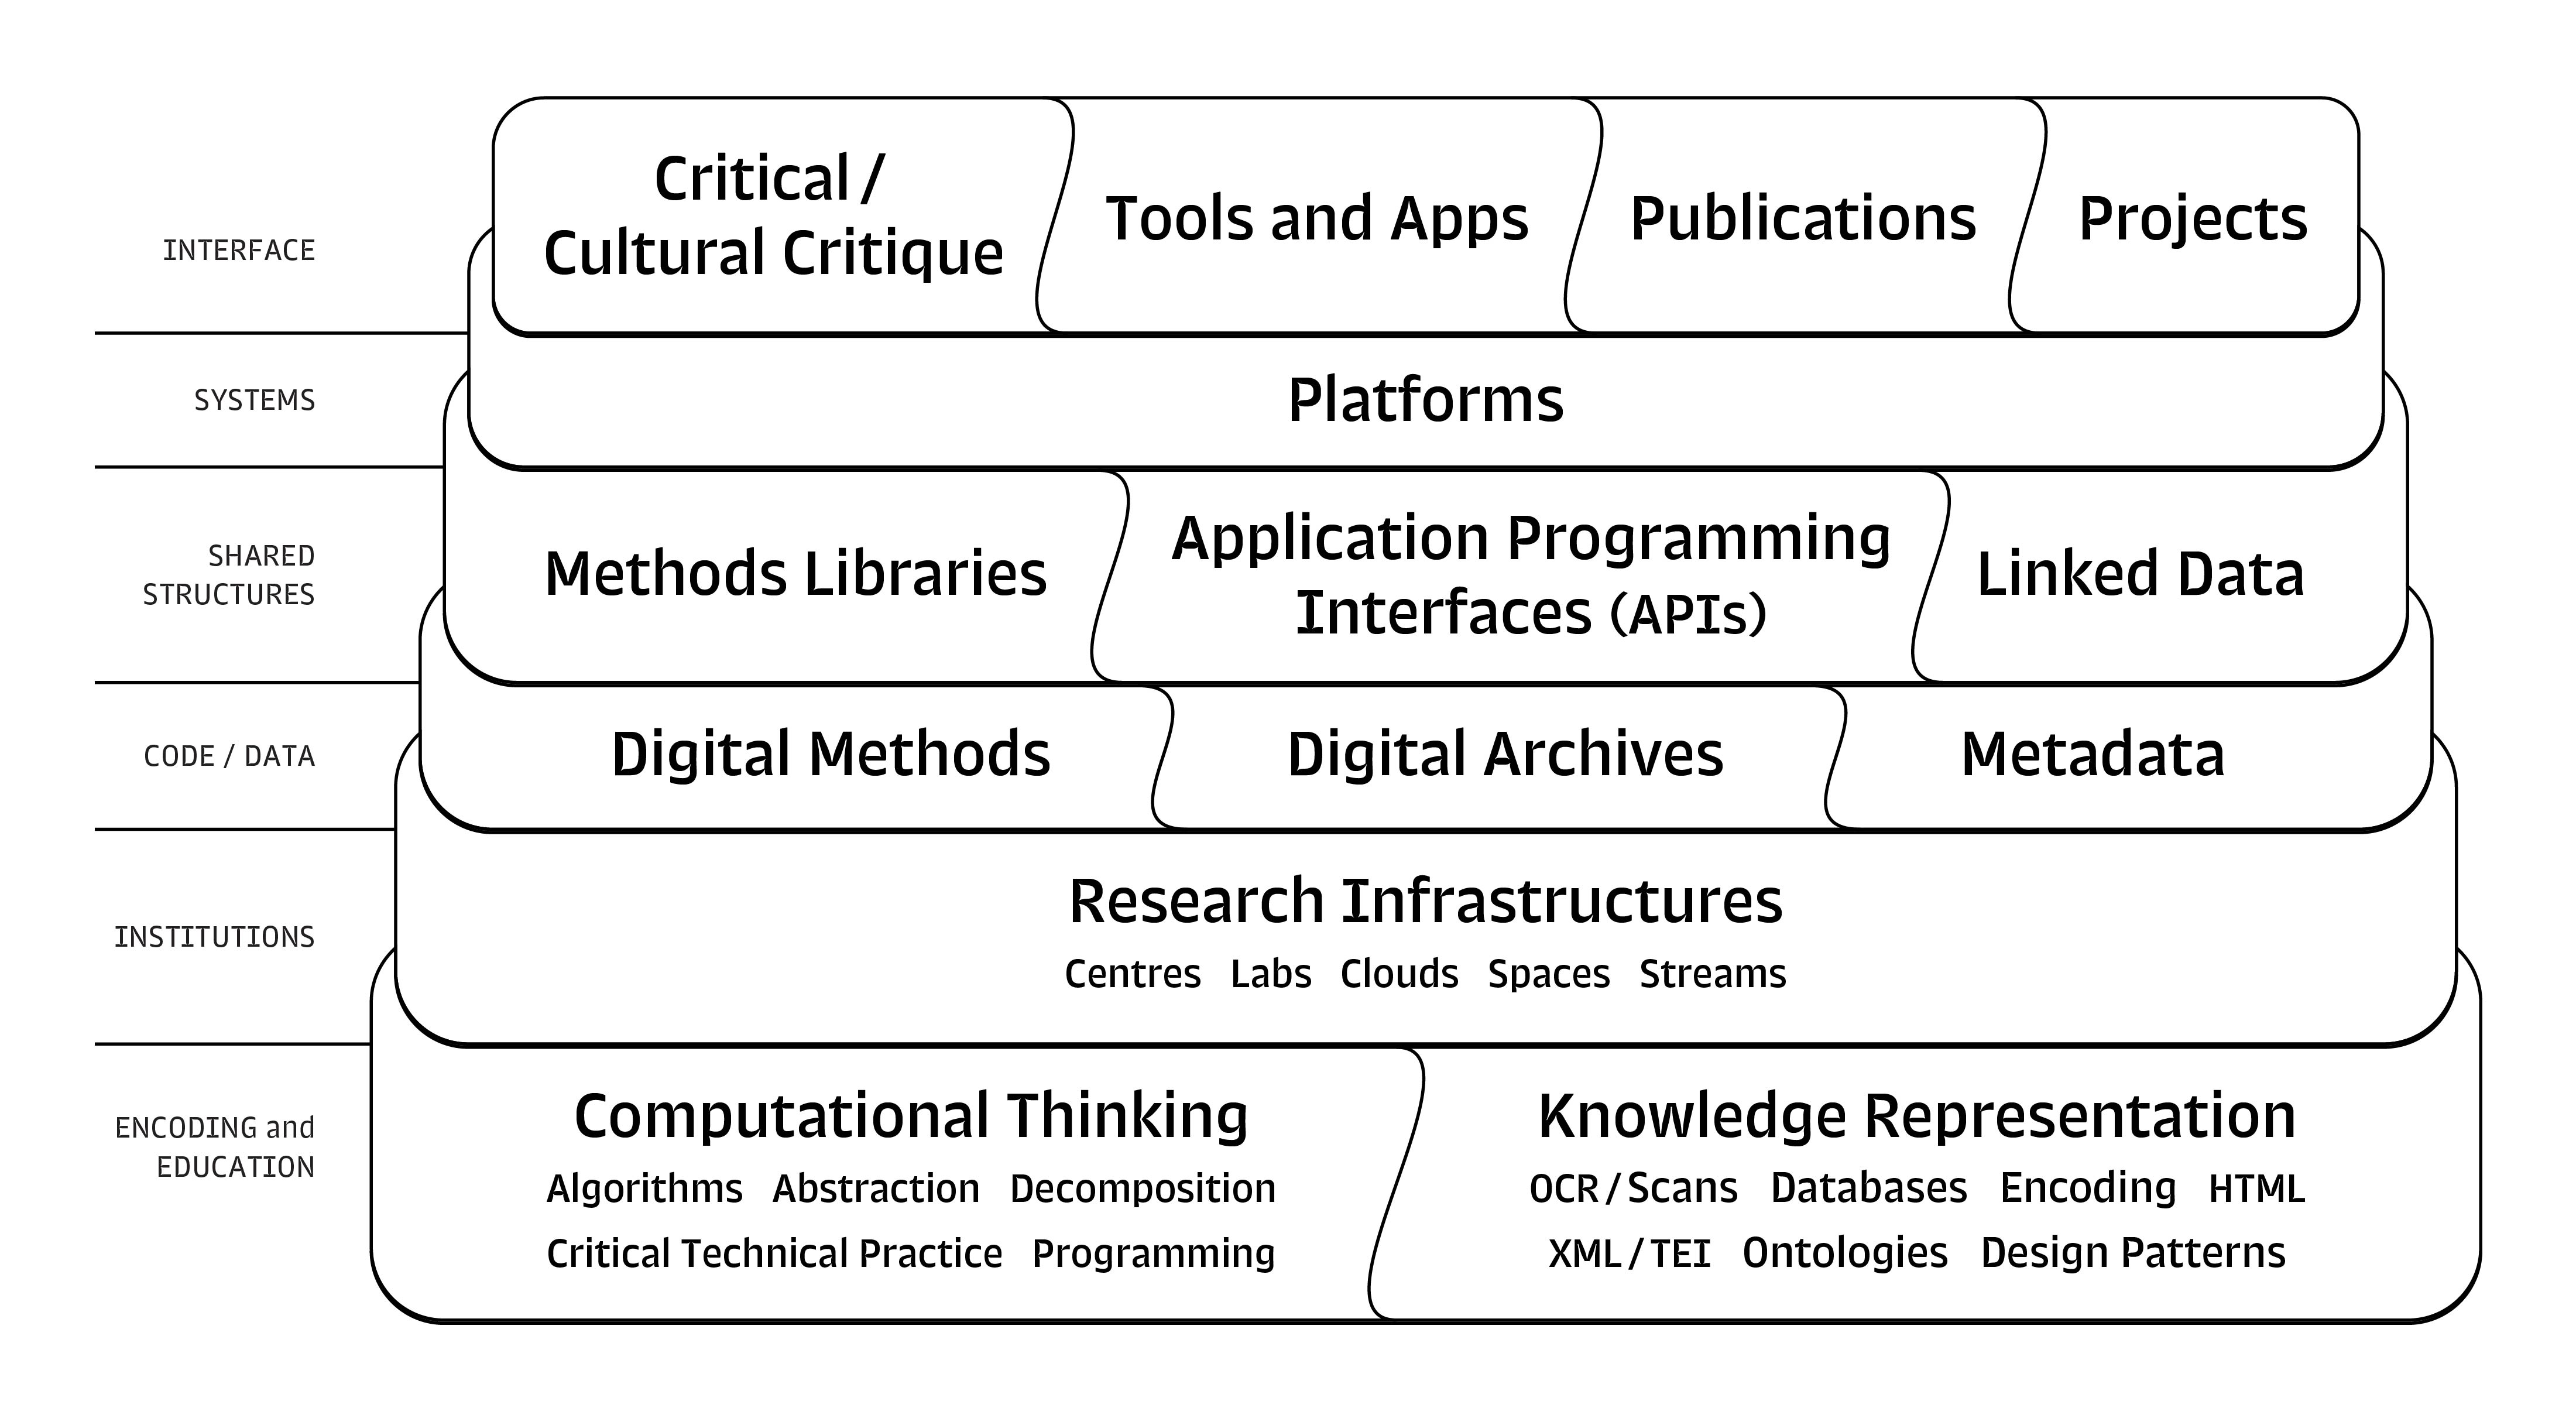
\includegraphics[width=.9\textwidth]{Digital_Humanities_Stack_(from_Berry_and_Fagerjord_2017-_18)}
\end{frame}

\begin{frame}
  \frametitle{Институционализация}

  \begin{itemize}
    \item 1966~--- журнал \textit{Computers and the Humanities}
    \item 1973~--- ассоциация \textit{Computer Applications and Quantitative Methods in Archaeology}
    \item 1977/78~--- \textit{Association for Literary and Linguistic Computing / Computers and the Humanities}
  \end{itemize}
\end{frame}

\begin{frame}
  \frametitle{Примеры проектов}

  \begin{block}{Index Thomisticus}
    \begin{itemize}
      \item проект священника Роберто Буса, поддержанный IBM
      \item 179 текстов о Фоме Аквинском, 10 млн словоформ
    \end{itemize}
  \end{block}

  \vfill

  \begin{itemize}
    \item Факсимильные копии ОР РНБ: \linebreak \url{http://nlr.ru/manuscripts}
    \item База данных <<Пермская губернская периодика: 1914--1922>>: \linebreak \url{http://permnewspapers.ru/}
  \end{itemize}
\end{frame}

\begin{frame}
  \frametitle{TEI}
  \framesubtitle{Фрагмент разметки}

  \begin{center}
    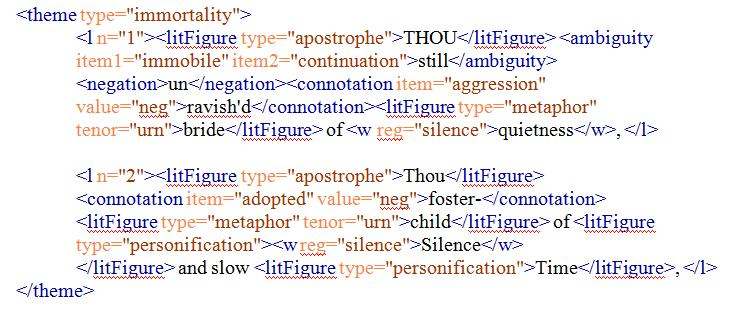
\includegraphics[width=\linewidth]{tei}
  \end{center}
\end{frame}

\begin{frame}
  \frametitle{TEI}
  \framesubtitle{Примеры глав}

  \begin{itemize}
    \item Verse; Performance Texts; Transcriptions of Speech
    \item Manuscript Description; Representation of Primary Sources; Critical Apparatus
    \item Tables, Formulæ, Graphics, and Notated Music
  \end{itemize}
\end{frame}
